%%*************************************************************************
%% The Berkeley Out-of-Order Machine
%% Christopher Celio
%% 2015 Dec 17
%% 
%% Design document
%%*************************************************************************


\documentclass[11pt, notitlepage]{report}


\usepackage{graphicx}
\usepackage{url}
\usepackage{fullpage}
\usepackage{listings} % used for putting code
\usepackage{color}
\usepackage[multiple]{footmisc}
%\usepackage{wrapfig} % allow text to wrap around a figure

\usepackage{hyperref} 
\hypersetup{
    colorlinks=true,
    linkcolor=black,
    urlcolor=red,
    citecolor=black,
    filecolor=black,
    linktoc=all
}

\let\tt\texttt

\lstset{ %
language=C++,                % choose the language of the code
%basicstyle=\small\ttfamily,      % the size of the fonts that are used for the code
basicstyle=\scriptsize\ttfamily,basewidth=0.50em,      % the size of the fonts that are used for the code
numbers=left,                   % where to put the line-numbers
numberstyle=\scriptsize,      % the size of the fonts that are used for the line-numbers
stepnumber=1,                   % the step between two line-numbers. If it is 1 each line will be numbered
numbersep=5pt,                  % how far the line-numbers are from the code
backgroundcolor=\color{white},  % choose the background color. You must add \usepackage{color}
showspaces=false,               % show spaces adding particular underscores
showstringspaces=false,         % underline spaces within strings
showtabs=false,                 % show tabs within strings adding particular underscores
frame=single,                   % adds a frame around the code
tabsize=3,              % sets default tabsize to 3 spaces
captionpos=b,                   % sets the caption-position to bottom
breaklines=true,        % sets automatic line breaking
breakatwhitespace=false,    % sets if automatic breaks should only happen at whitespace
linewidth=1.0\textwidth,
boxpos=b,
%escapeinside={\%
%}
%{
%)}          % if you want to add a comment within your code
}
\renewcommand{\lstlistingname}{Code} % change caption title from 'listings' to what I want



\newcommand{\smalltodo}[1]{\marginpar{\footnotesize #1}}

\newcommand{\TODO}[1]{{\color{red} {\textbf [ TODO: #1 ]}}}
\newcommand{\fixme}[1]{{\color{red} {\textbf [ FIXME: #1 ]}}}
\newcommand{\ooo}{out-of-order}
\newcommand{\boom}{{\em BOOM}}
\newcommand{\BOOM}{{\em BOOM}}
\newcommand{\Chisel}{{\em Chisel}}
\newcommand{\Rocket}{{\em Rocket}}
\newcommand{\rocket}{{\em Rocket}}
\newcommand{\rocketchip}{{\em Rocket-chip}}
\newcommand{\fdiv}{{\tt {fdiv}}}
\newcommand{\ghistory}{{\em {ghistory}}}
\newcommand{\jal}{{\tt {JAL}}}
\newcommand{\jalr}{{\tt {JALR}}}


% allow us to add comentary
\newenvironment{commentary}
{ \vspace{-0.2in}
  \begin{quotation}
  \noindent
  \small \em
  \rule{\linewidth}{1pt}\\
}
{
  \end{quotation}
  \vspace{-0.2in}
}



\let\oldthebibliography=\thebibliography
\let\endoldthebibliography=\endthebibliography
\renewenvironment{thebibliography}[1]{%
  \begin{oldthebibliography}{#1}%
    \setlength{\parskip}{0ex}%
    \setlength{\itemsep}{0ex}%
  }%
  {%
    \end{oldthebibliography}%
  }

%%*************************************************************************
\begin{document}


\title{The Berkeley Out-of-Order Machine (BOOM) Design Specification}
\author{Christopher Celio, David Patterson, and Krste Asanovi\'{c}\\
%School of Electrical and Computer Engineering\\
University of California, Berkeley, California 94720--1770\\
{\tt celio@eecs.berkeley.edu}}

\maketitle

%%*************************************************************************

\

\

{\centerline {\color{red}This draft is a work-in-progress.}}


\vfill

\hrule
\

\noindent The information in this publication is subject to change without notice. 

\noindent This document is available at: \url{https://ccelio.github.io/riscv-boom-doc}.

\

\noindent Copyright \copyright\ 2016 Christopher Celio

\

\noindent This work is licensed under the Creative Commons Attribution 4.0 International License (CC BY 4.0). To view a copy of this license, visit \url{http://creativecommons.org/licenses/by/4.0/}.


\thispagestyle{empty} % suppress page number 

%%*************************************************************************

\tableofcontents

\include{sections/intro}
\include{sections/fetch}
\include{sections/bpd}
\include{sections/decode}
\include{sections/rename}
\include{sections/rob}
\include{sections/issue}
\include{sections/registerread}
\include{sections/execute}
\include{sections/lsu}
\include{sections/memory}
\include{sections/uarch-counters}
\include{sections/verification}
\chapter{Debugging}
\include{sections/visualization}
\include{sections/physical}
\appendix
\include{sections/futurework}
\include{sections/parameterization}

\chapter{Frequently Asked Questions}

To be filled in as questions are asked!

\include{sections/terminology}


\begin{figure}[ht]
	\centering
	\centerline{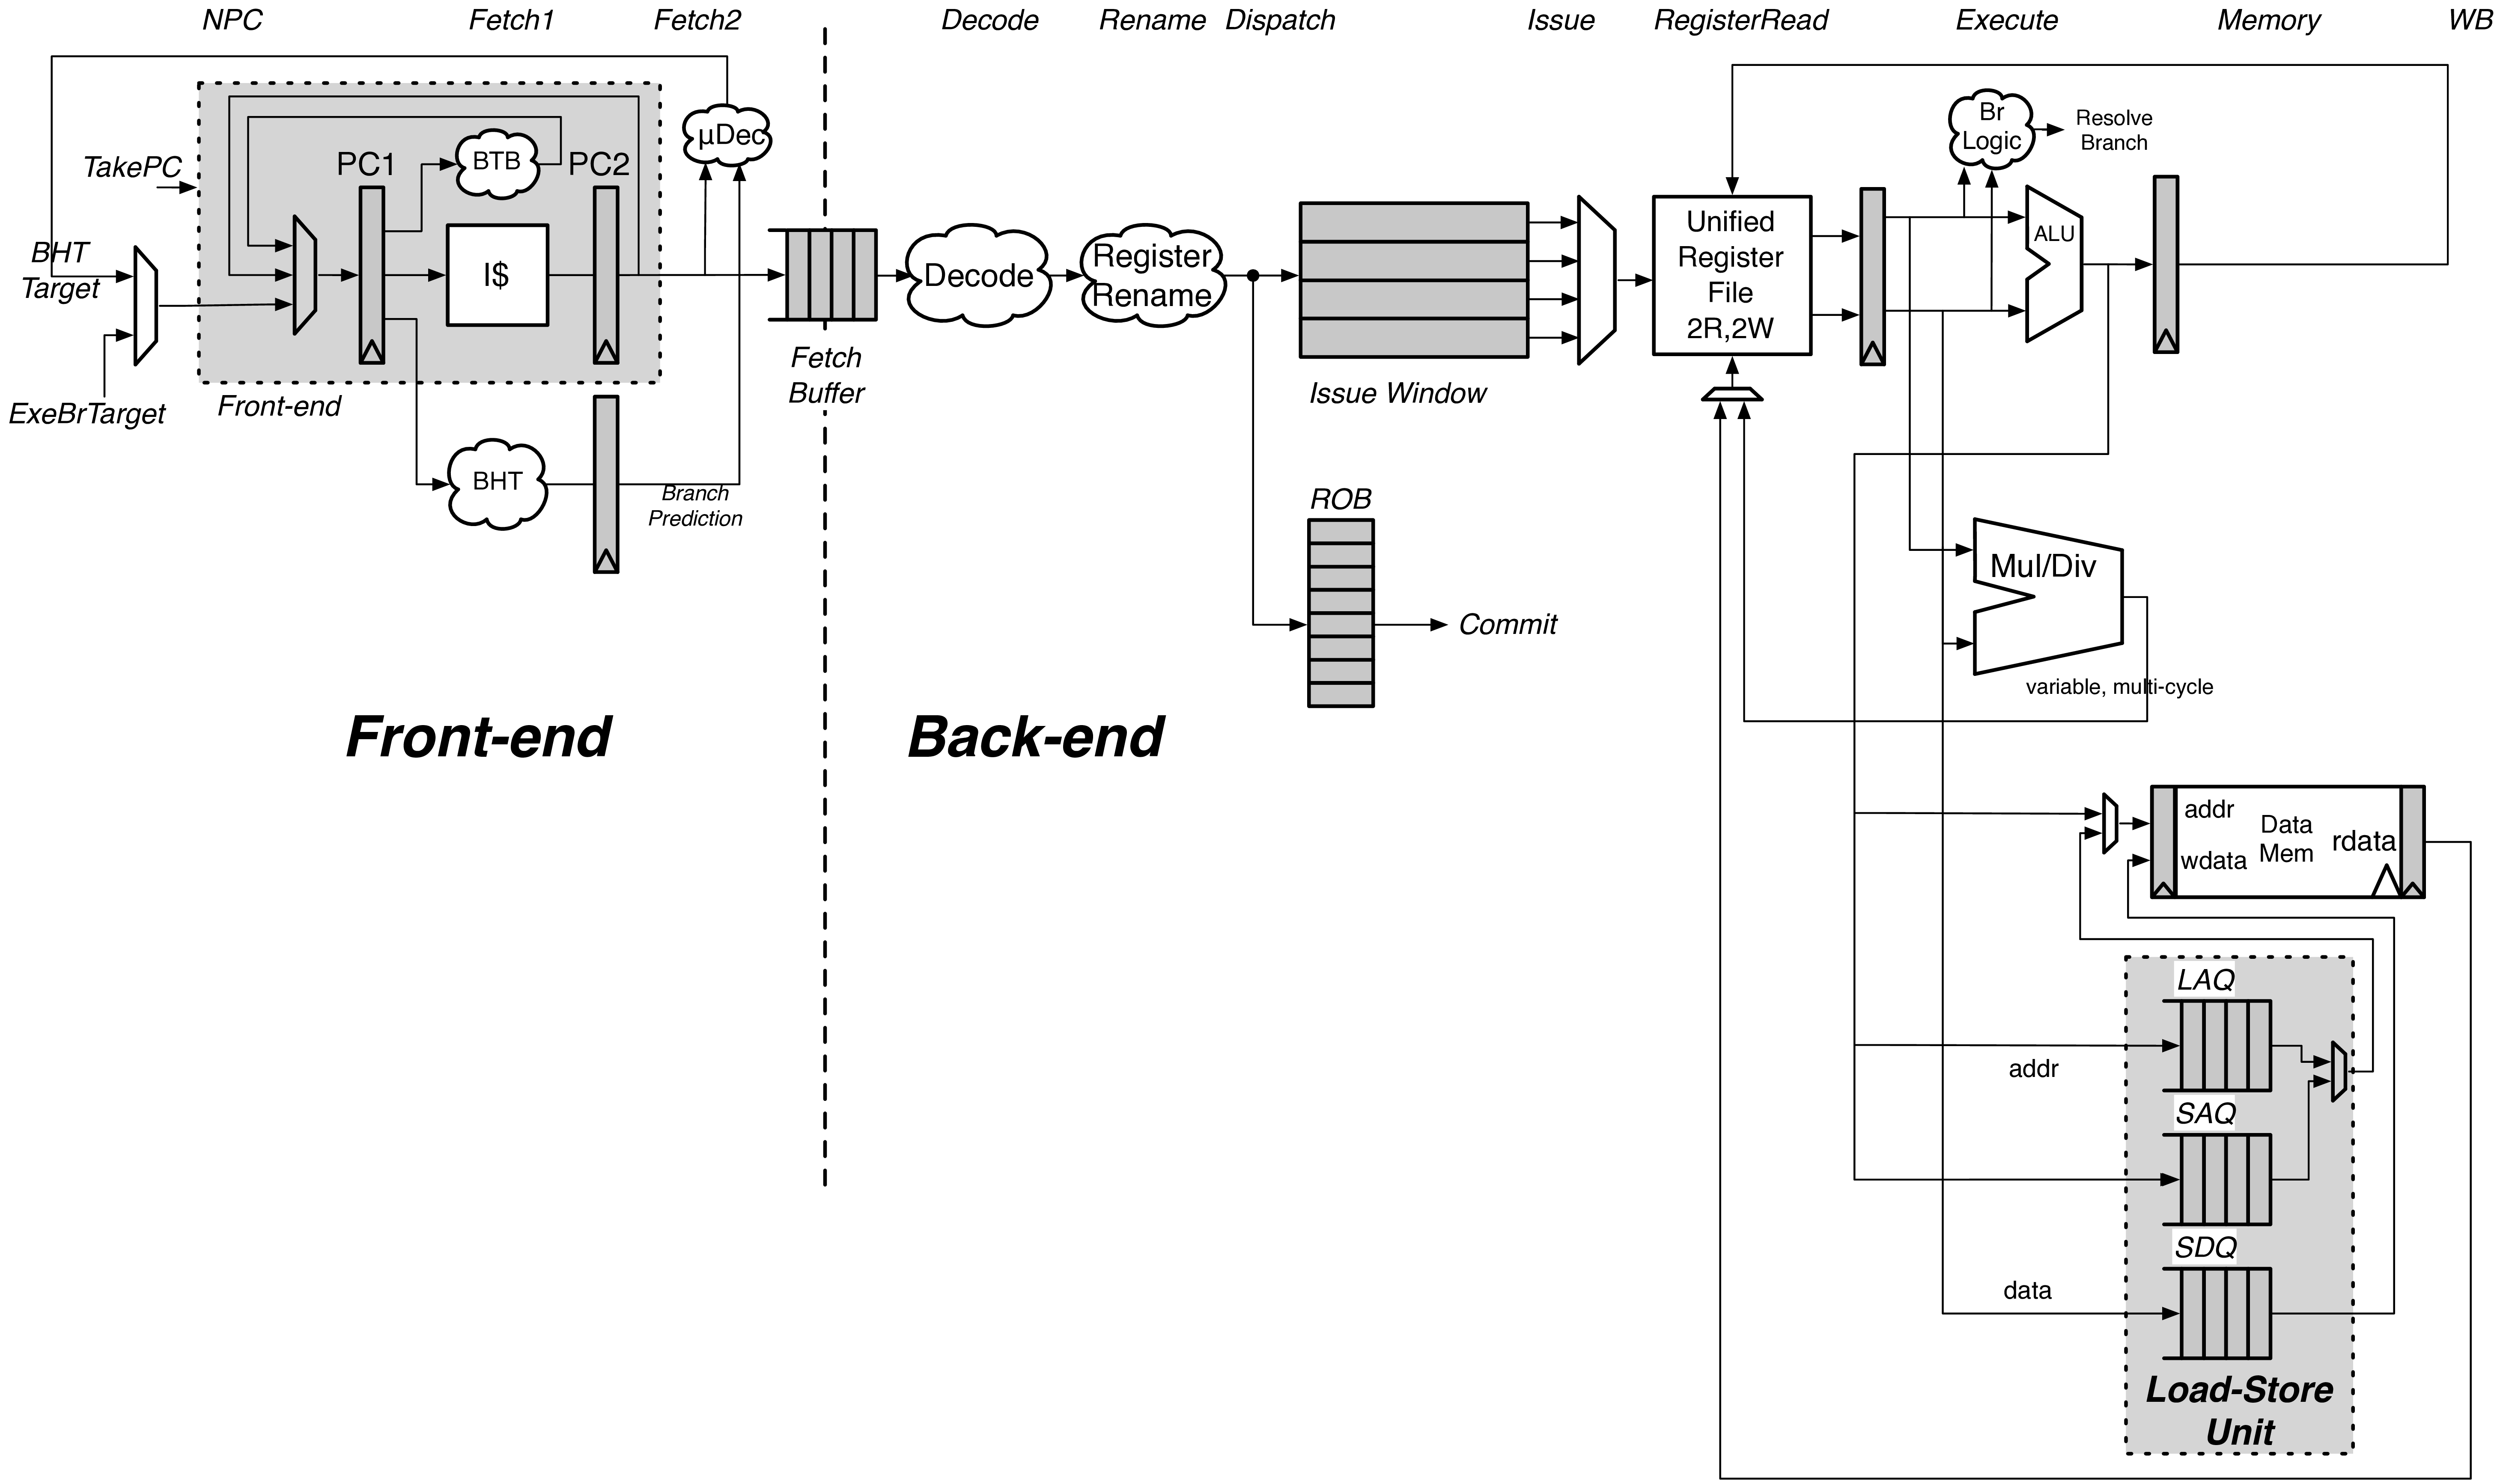
\includegraphics[scale =.9, angle=90] {figures/simple_boom_pipeline}}
	\caption{ \small A more detailed diagram of BOOM, for a single-issue RV32IM design.}
	\label{fig:boom-detailed}
\end{figure}






%\begin{scriptsize}
\bibliographystyle{abbrv}
\bibliography{bibliography}
%\end{scriptsize}


\end{document}
